\chapter{Examples}

In the following sections, three example problems are demonstrated using the proposed algorithm to compute a CBF-QP controller. Section \ref{sec:platooning} demonstrates a convoy of platooning vehicles, to illustrate a more abstract example of OKC systems. Section \ref{sec:drone} demonstrates a drone navigating in the presence of obstacles, to show application to under-actuated systems. Finally, section \ref{sec:7dof} demonstrates a seven-degree of freedom manipulator, to show realtime performance on a chaotic high degree of freedom system.



\section{Platooning} \label{sec:platooning}
\noindent A commonly cited use case for control barrier functions is platooning. In this application, a set of vehicles traveling along a road which to reach a desired speed while maintaining adequate stopping distance. 
\begin{figure}[H]
    \centering
    \includegraphics[width=\textwidth]{Figures/Examples/Platoon/Platoon.png}
    \caption{Platooning Busses}
    \label{fig:platoon_diag}
\end{figure}
\noindent Such a system as a series of prismatic joints all attached to one common root. The root joint is an inertial frame at $x=0$.  

\begin{figure}[H]
    \centering
    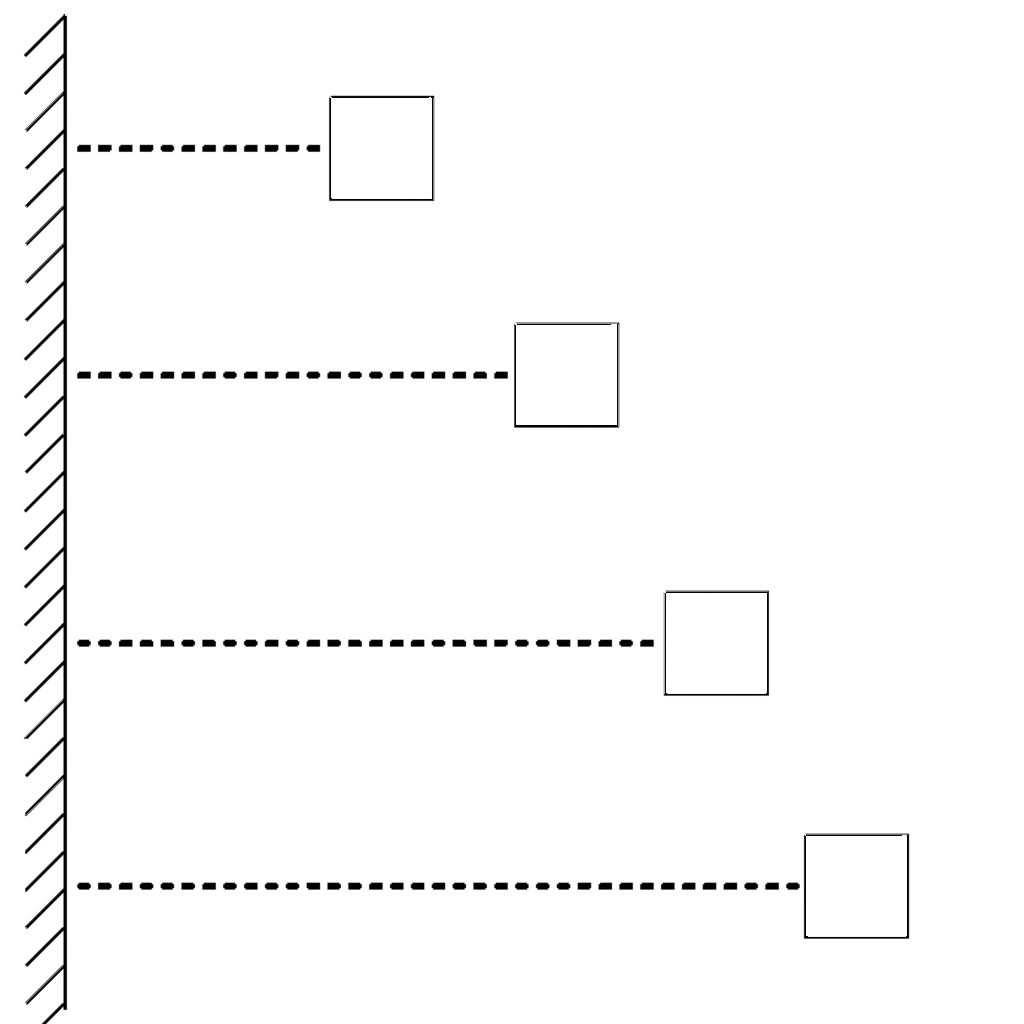
\includegraphics[width=0.4\textwidth]{Figures/Examples/Platoon/PlatoonNE.png}
    \caption{Platooning OKC Model}
    \label{fig:platoon_diag_2}
\end{figure}
\noindent A four vehicle platoon will now be demonstrated. All vehicles have mass $m = 1$, and are children of the inertial frame. 
\subsection{Reference Controller}
\noindent The system will include a reference P controller that aims to get all vehicles to a desired speed, $v_d$.
\begin{align} \label{eqn:platoon_reference}
    u = v_d - \dotx
\end{align}
\noindent Figure \ref{fig:platoon_no_cbf} shows the response of the system starting from $x_0 = [1 \quad 2 \quad 3 \quad 4]$, $v_d = 10$ with no safety controller.

\begin{figure}[H]
    \centering
    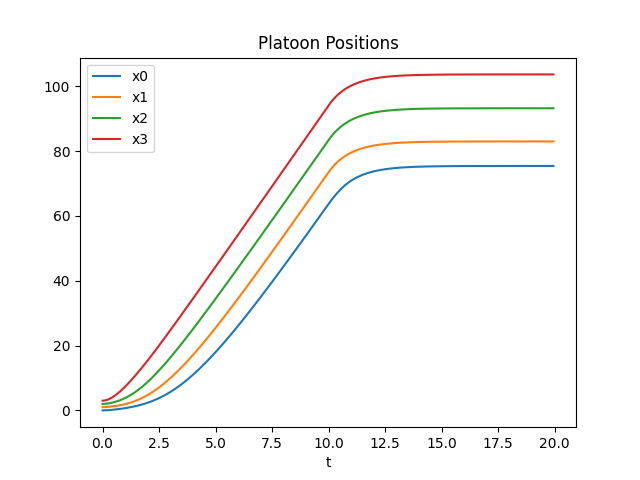
\includegraphics[width=0.45\textwidth]{Figures/Examples/Platoon/NoPositions.png}
    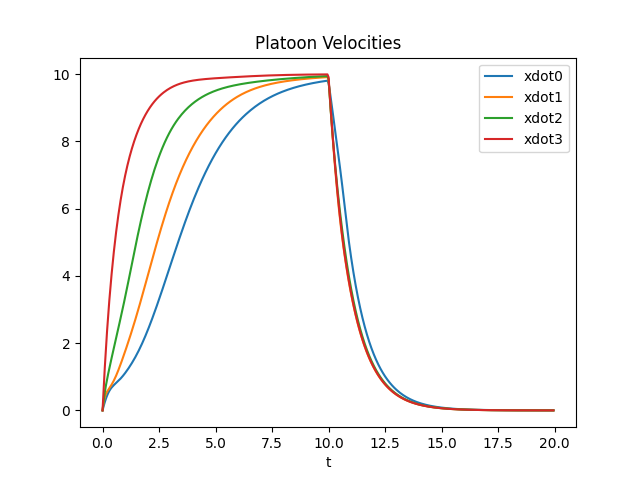
\includegraphics[width=0.45\textwidth]{Figures/Examples/Platoon/NoVelocities.png}
    \caption{Platoon Response Without CBF}
    \label{fig:platoon_no_cbf}
\end{figure}

\noindent While all vehicle reach the desired speed, many would consider this to be an unsafe platoon as the stopping distance between vehicles decreases as speed increases. To combat this, a barrier can be added, mandating at least 1 second of stopping time between adjacent vehicles. This is given by the equation,
\begin{align*}
    h(\x, \dotx) = \prod_{i = 0}^3 ((\x_{i + 1} - \x_i) -  \dotx_i)
\end{align*}
\noindent Figure \ref{fig:platoon_cbf} shows the response of the system with the same reference controller, this time enforcing the CBF.
\begin{figure}[H]
    \centering
    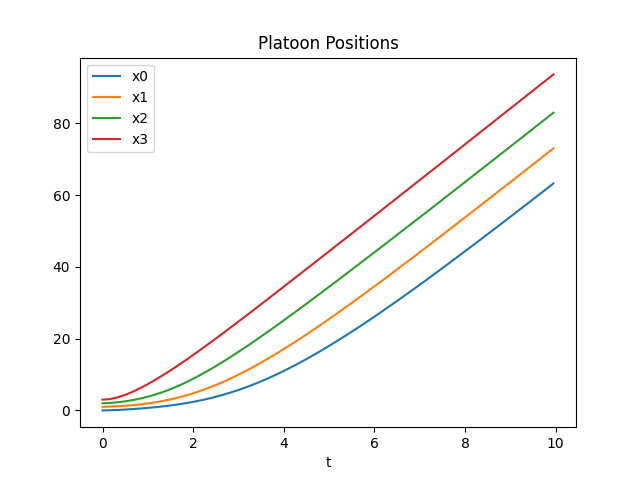
\includegraphics[width=0.4\textwidth]{Figures/Examples/Platoon/Positions.png}
    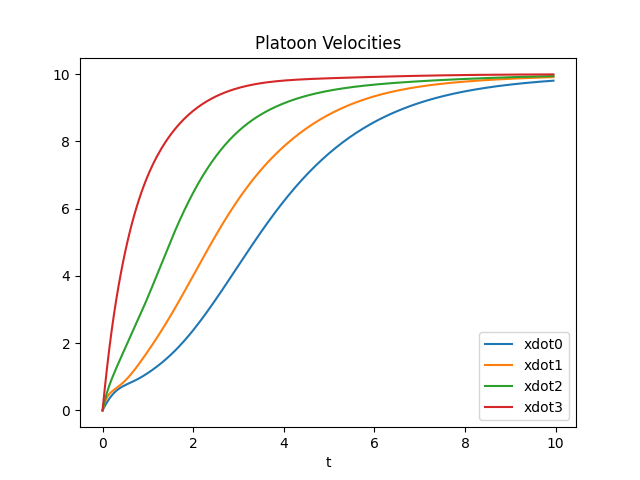
\includegraphics[width=0.4\textwidth]{Figures/Examples/Platoon/Velocities.png}
    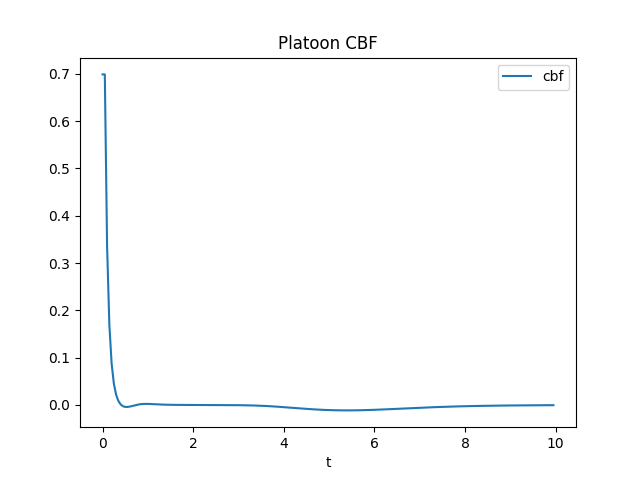
\includegraphics[width=0.4\textwidth]{Figures/Examples/Platoon/CBF.png}
    \caption{Platoon Response With CBF}
    \label{fig:platoon_cbf}
\end{figure}
\noindent Unlike the first example, the vehicles now separate to maintain adequate stopping time as they accelerate. Vehicles still accelerate when able, and eventually all vehicles reach the target velocity.
\section{Drone Cave Navigation}  \label{sec:drone}

\noindent To demonstrate an underactuated system, we will model a simple drone in two dimensions.

\begin{figure}[H]
    \centering
    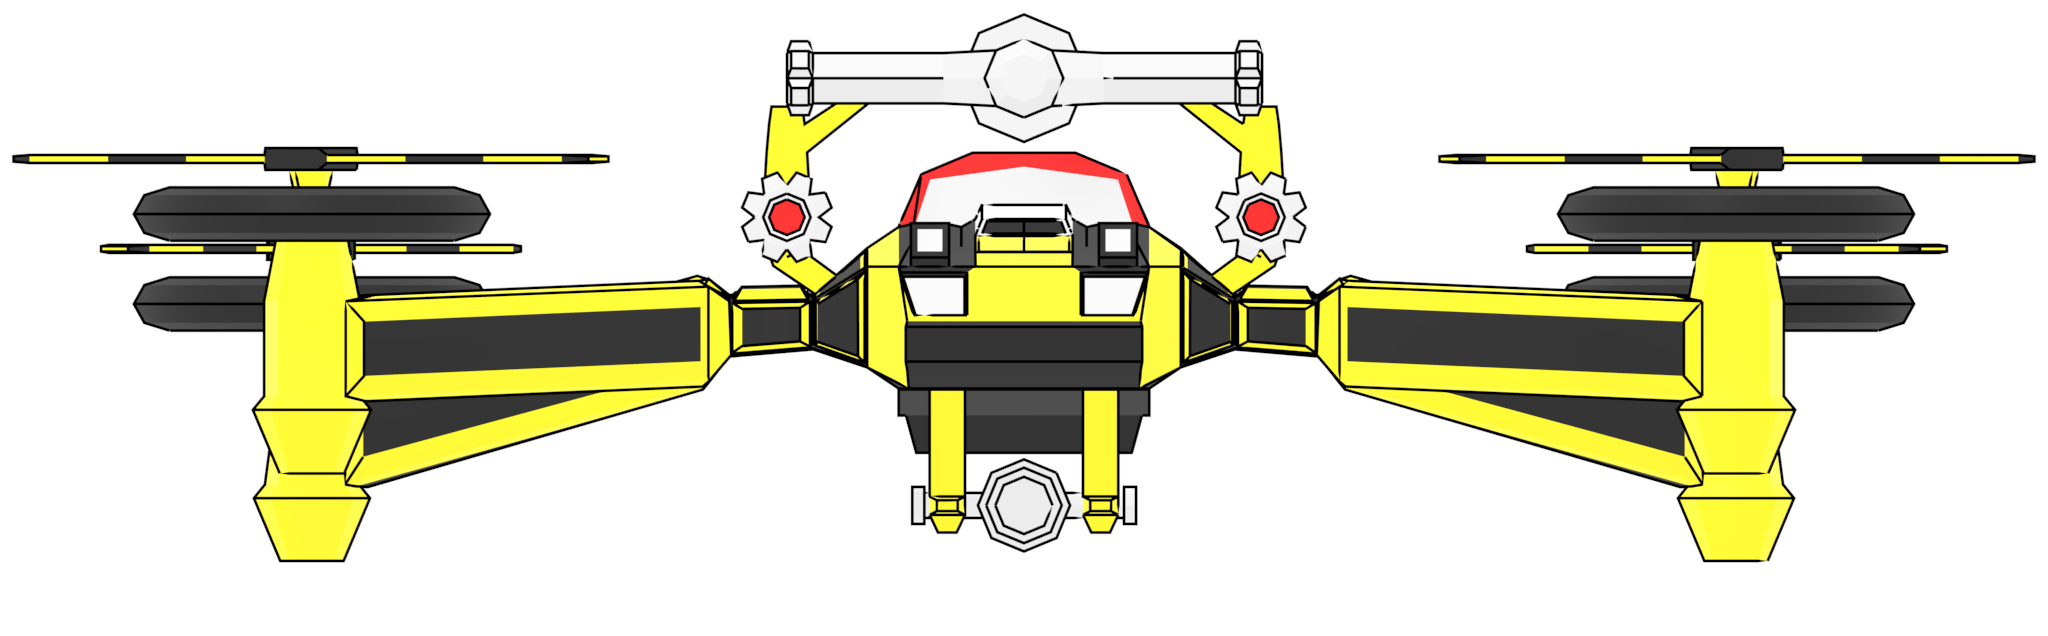
\includegraphics[width=0.4\textwidth]{Figures/Examples/Drone/Drone.jpg}
    \caption{Drone Free Body Diagram}
    \label{fig:drone}
\end{figure}
\noindent We can model this system as 3 separate bodies with the following properties.
\begin{align*}
    \begin{split}
        {^I_I \r _0} &= \begin{bmatrix} x & 0 & 0\end{bmatrix} \\
        {^0_0 \r _1} &= \begin{bmatrix} 0 & y & 0 \end{bmatrix} \\ 
        {^1_1 \r _2} &= \begin{bmatrix} 0& 0& 0 \end{bmatrix}\\
    \end{split}
    \begin{split}
        {^I \T_0} &= \EYE\\
        {^0 \T_1} &= \EYE\\
        {^1 \T_2} &= \text{rotz}(\theta)\\
    \end{split}
    \begin{split}
    \end{split}
    \begin{split}
        {^0_0 \com _0} &= \begin{bmatrix} 0& 0& 0 \end{bmatrix}\\
        {^1_1 \com _1} &= \begin{bmatrix} 0& 0& 0 \end{bmatrix}\\
        {^2_2 \com _2} &= \begin{bmatrix} 0& 0& 0 \end{bmatrix}\\
    \end{split}
\end{align*}
\begin{figure}[H]
    \centering
    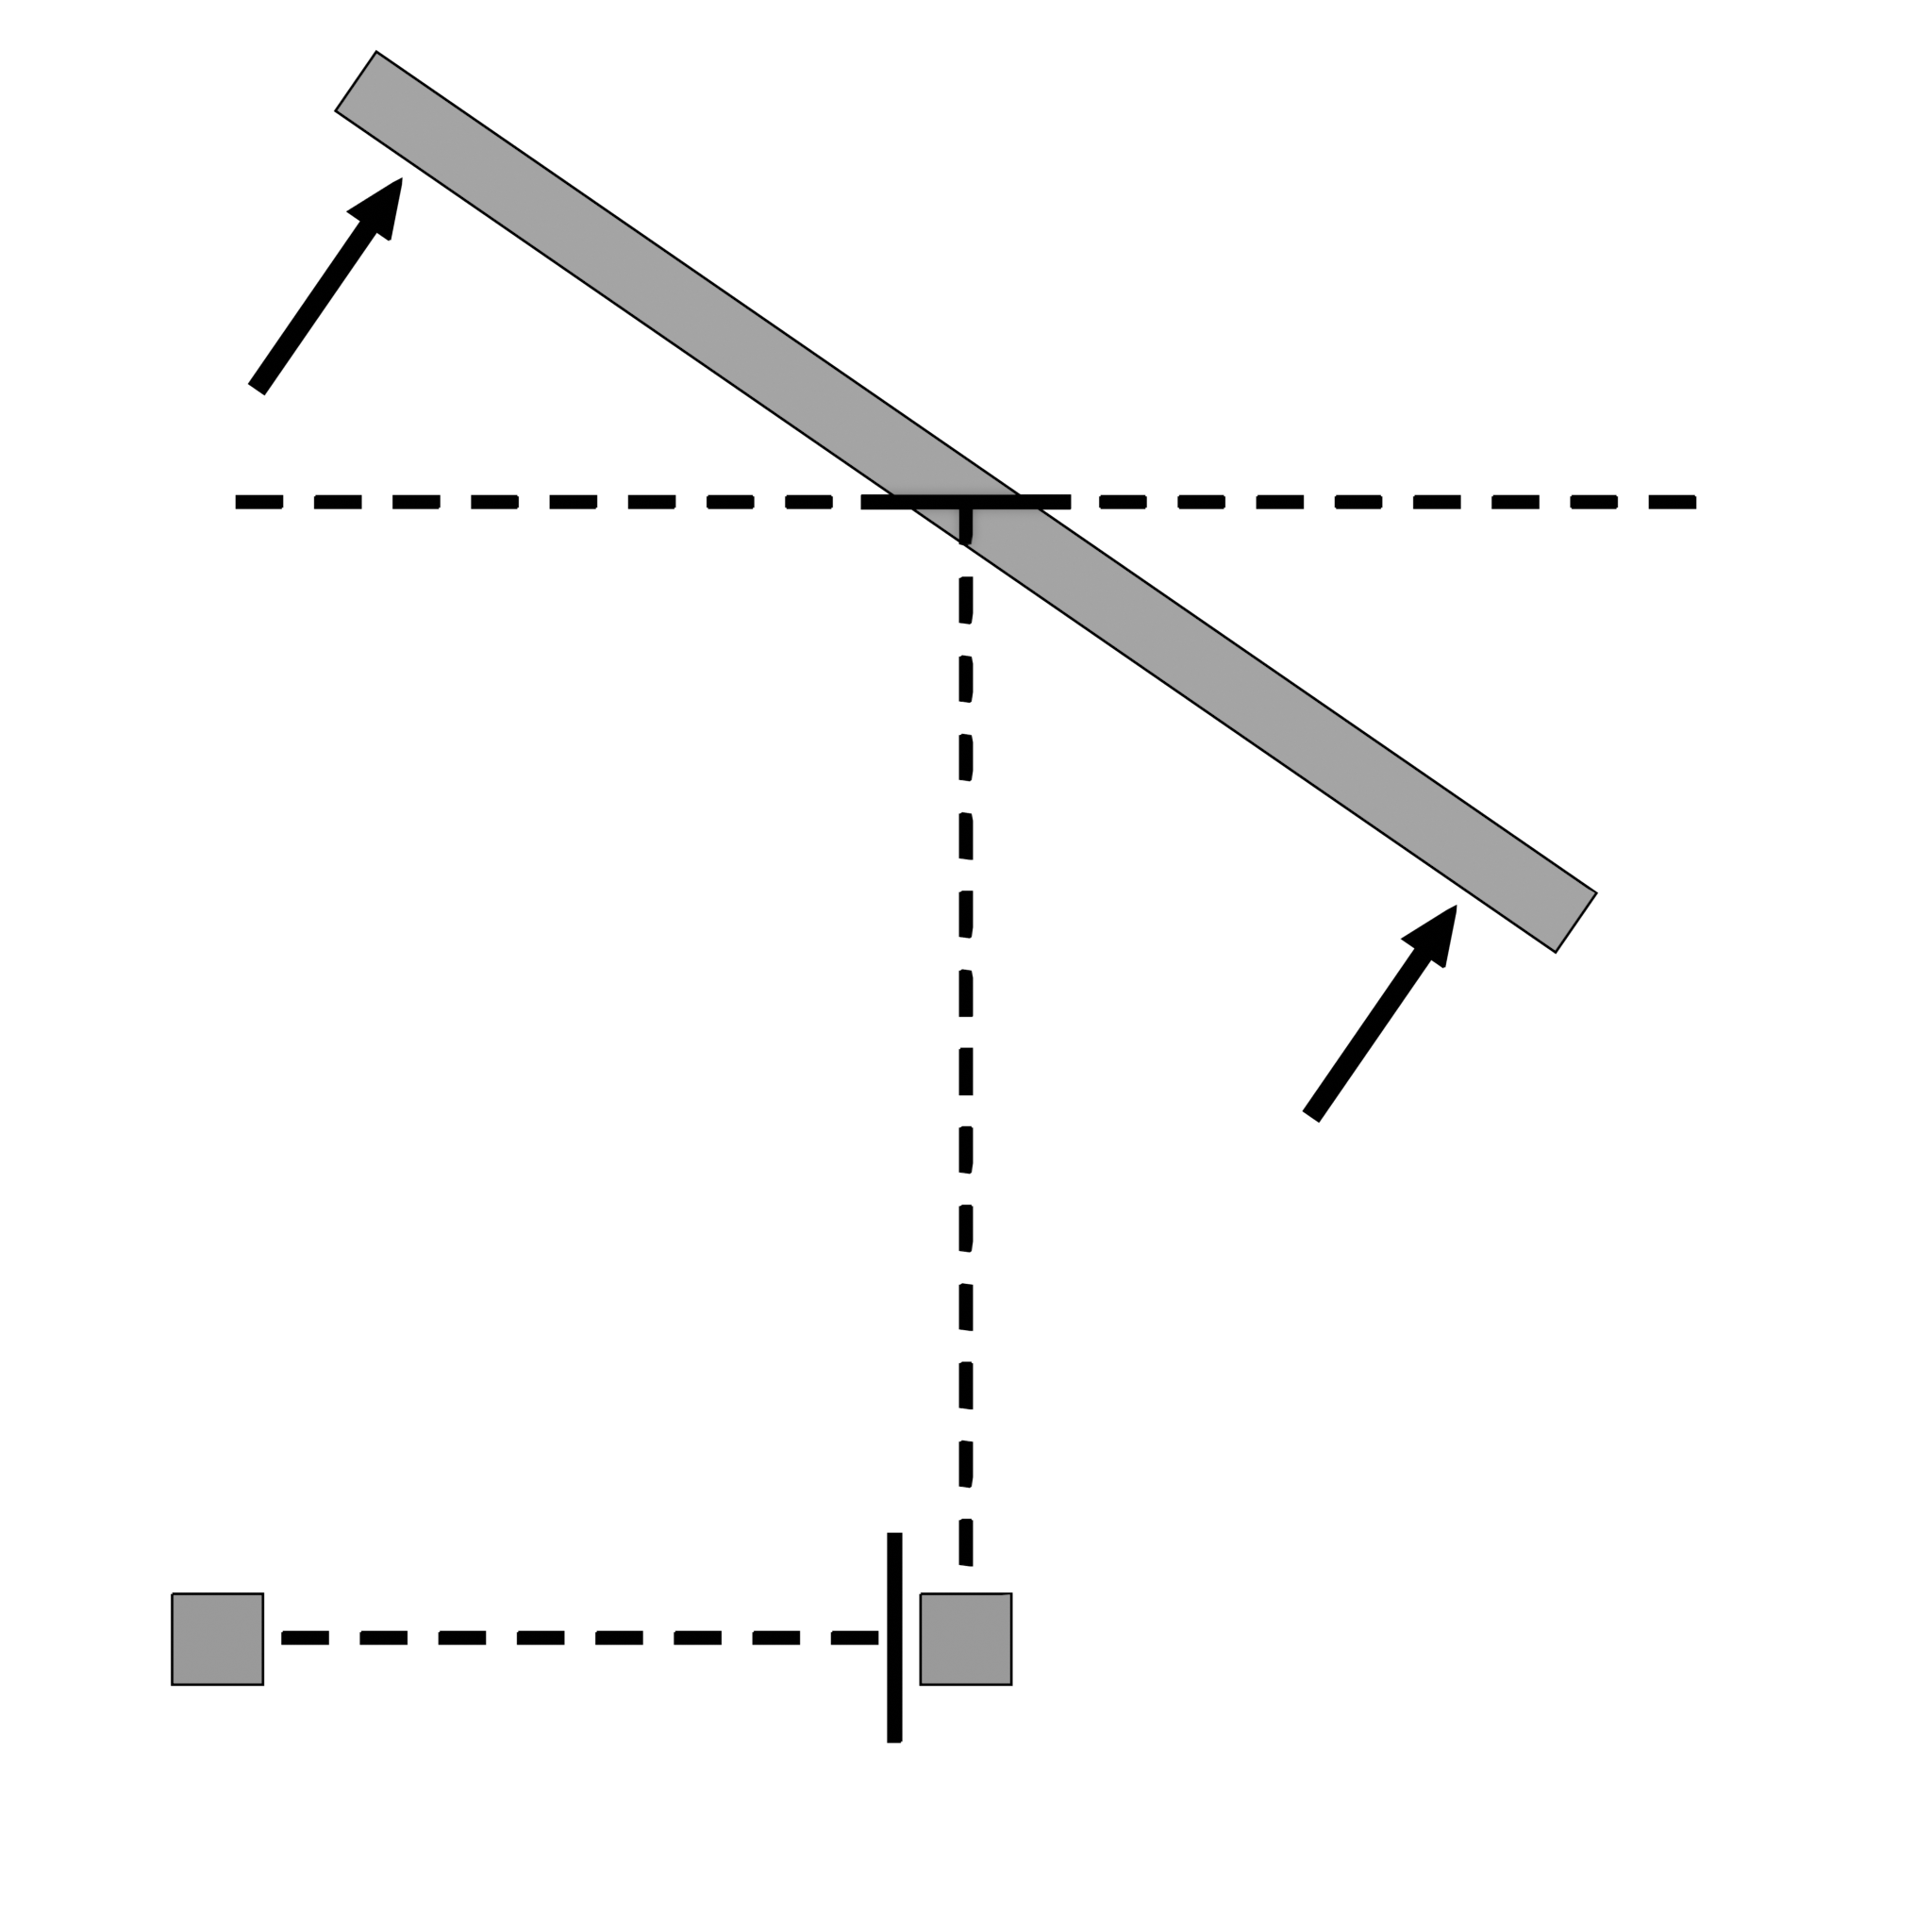
\includegraphics[width=0.4\textwidth]{Figures/Examples/Drone/DroneNE.png}
    \caption{Drone OKC Model}
    \label{fig:drone}
\end{figure}
\noindent The force of the propellers $\left [ u_1 \quad u_2 \right ]$ is projected into the joint space with the following input matrix
\begin{align*}
    \P(x, y, \theta) = \begin{bmatrix}
    -r\sin{\theta} & -r\sin{\theta} \\ 
    r\cos{\theta} & r\cos{\theta} \\ 
    1 & -1 
    \end{bmatrix}
\end{align*}
\noindent We begin by deriving a reference controller that achieves a desired lateral and vertical position. This is broken into two separate controllers, positioning in each direction. 
\begin{align}
    u_{\text{vert}_1} = u_{\text{vert}_2} &= \frac{g}{2 \cos{\theta}} + P_{\text{vert}} \left (y_{\text{goal}} -  y\right) - D_{\text{vert}}\dot{y} \\
    u_{\text{lat}_2} = -u_{\text{lat}_1} &= P_{\text{lat}_1}\arctan{\left ((1 - D_{\text{lat}_1})\dot{x} - (x_{\text{goal}} - x) \right )} -  P_{\text{lat}_2}\theta - D_{\text{lat}_2}\dot{\theta}
\end{align}
\subsection{Reference Controller Performance}

\noindent We set the following control parameters:
\begin{align*}
\begin{split}
    P_{\text{vert}} &= 1 \\
    D_{\text{vert}} &= 3
\end{split}
\begin{split}
    P_{\text{lat}_1} &= 1 \\
    D_{\text{lat}_1} &= 1.5
\end{split}
\begin{split}
\end{split}
\begin{split}
    P_{\text{lat}_2} &= 5 \\
    D_{\text{lat}_2} &= 5
\end{split}
\end{align*}

\noindent Figure \ref{fig:dronepd} shows the path the drone takes using this controller, starting from $(x, y, \theta) = (0, 0, 0)$ to reach $(5, 5, 0)$.

\begin{figure}[H]
    \centering
    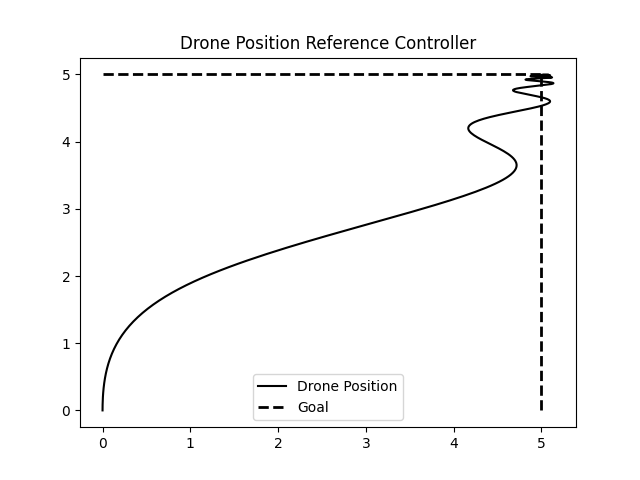
\includegraphics[width=0.5\textwidth]{Figures/Examples/Drone/DronePD.png}
    \caption{Drone Path Reference Control}
    \label{fig:dronepd}
\end{figure}

\noindent While the drone does not significantly overshoot the target position, there is overshoot on the intermediate path. However, we will see that with a CBF implemented we can avoid obstacles even with this overshoot. On the test system, this controller ran at an average 276.97Hz.

\subsection{Collision Avoidance}

\noindent In this challenge, the drone will attempt to navigate a cave modeled by a sinusoidal curve. The roof and floor of this cave are given by the following 
\begin{align}
    \begin{split}
        \text{Roof}(x) = \sin{x} + 1
    \end{split}
    \begin{split}
        \text{Floor}(x) = \sin{x} + 1
    \end{split}
\end{align}
\noindent We wish to enforce a safety buffer of 0.5 meters between the drone and boundaries of the cave. With this, we have the following barrier function
\begin{align}
    h(x, y, \theta) = (\text{Roof}(x) - y + 0.5)(y - 0.5 - \text{Floor}(x))
\end{align}
\noindent Before enforcing the barrier, we will first try a best effort approach. For this, we will use the existing reference controller, with a target height of $y = \sin{x}.$ Figure \ref{fig:DronePathNoCBF} shows a simulation of this best effort controller. 

\begin{figure}[H]
    \centering
    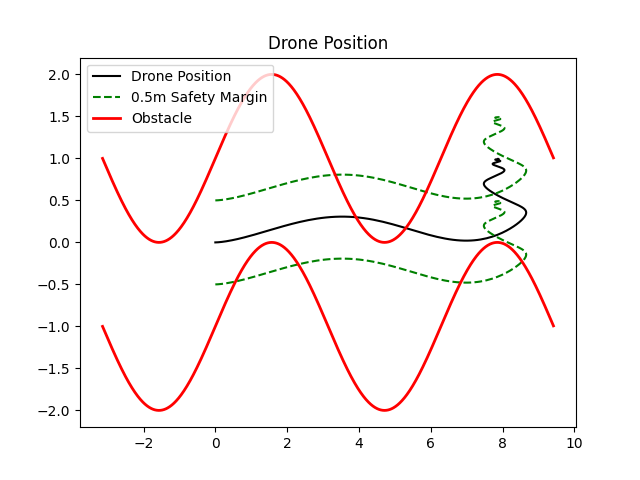
\includegraphics[width=0.45\textwidth]{Figures/Examples/Drone/DronePathNoCBF.png}
    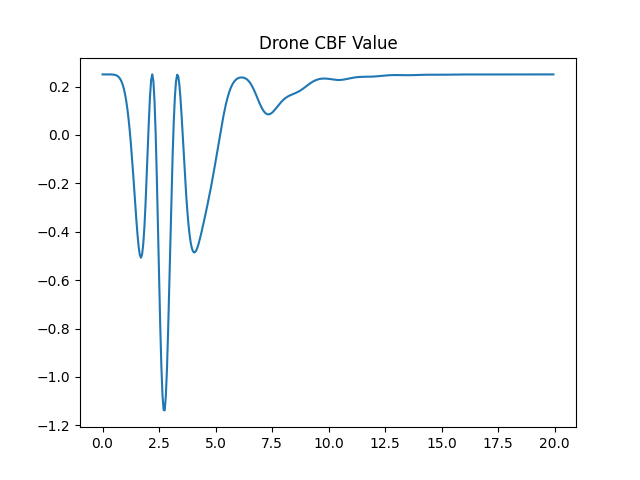
\includegraphics[width=0.45\textwidth]{Figures/Examples/Drone/DroneNoCBFValue.png}
    \caption{Drone: No CBF}
    \label{fig:DronePathNoCBF}
\end{figure}

\noindent Despite the target path being well within the safe set, the set is breached at several point in the simulation. Not just this, but the wall of the cave is breached as well. \newline

\noindent We now run the simulation again, this time enabling our control barrier function, in addition to our reference controller. The results of this simulation are shown in Figure \ref{fig:DronePathCBF}.

\begin{figure}[H]
    \centering
    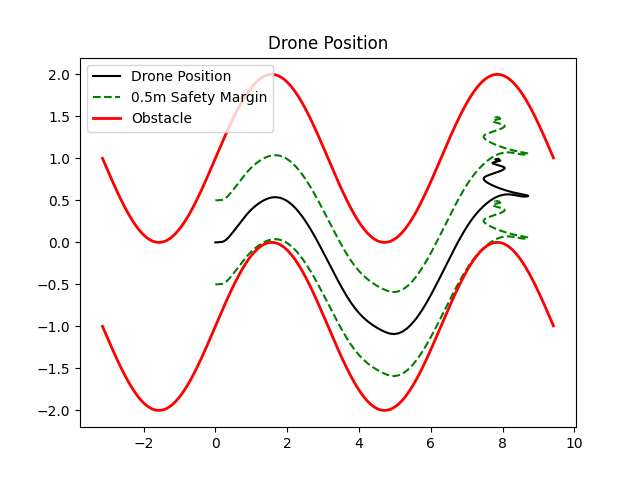
\includegraphics[width=0.45\textwidth]{Figures/Examples/Drone/DronePathCBF.png}
    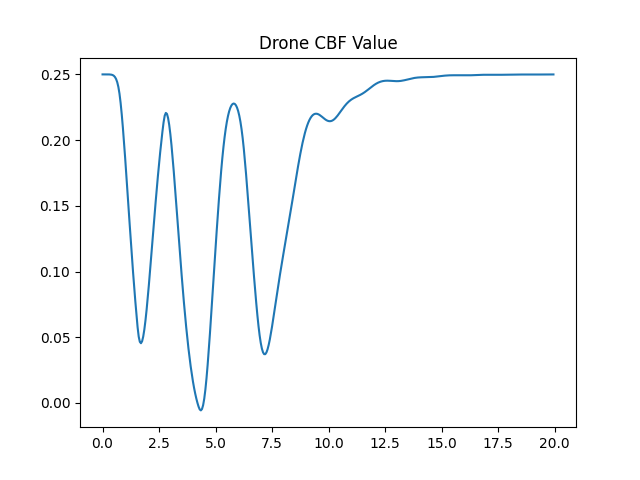
\includegraphics[width=0.45\textwidth]{Figures/Examples/Drone/DroneCBFValue.png}
    \caption{Drone: CBF}
    \label{fig:DronePathCBF}
\end{figure}
\section{7 DOF Manipulator}  \label{sec:7dof}

\noindent In this example we explore the the following 7DOF arm maniulator.

\begin{figure}[H]
    \centering
    \includegraphics[width=\textwidth]{Figures/Examples/7DOF Zeroed.png}
    \caption{7 DOF Zeroed}
    \label{fig:7dofzero}
\end{figure}

\begin{align*}
    \begin{split}
        {^I_I \r _0} &= \begin{bmatrix} 0 & 0 & 0\end{bmatrix} \\
        {^0_0 \r _1} &= \begin{bmatrix} 0 & 0 & 1 \end{bmatrix} \\ 
        {^1_1 \r _2} &= \begin{bmatrix} 0.5& 0.5& 0 \end{bmatrix}\\
        {^2_2 \r _3} &= \begin{bmatrix} 1& 0& 0 \end{bmatrix}\\
        {^3_3 \r _4} &= \begin{bmatrix} 0& -0.5& 0\end{bmatrix}\\
        {^4_4 \r _5} &= \begin{bmatrix} 1& 0& 0 \end{bmatrix}\\
        {^5_5 \r _6} &= \begin{bmatrix} 0 & 0.5 & 1 \end{bmatrix}
    \end{split}
    \begin{split}
        {^I \T_0} &= \text{rotz}(\theta_0)\\
        {^0 \T_1} &= \text{roty}(\theta_1)\\
        {^1 \T_2} &= \text{rotx}(\theta_2)\\
        {^2 \T_3} &= \text{roty}(\theta_3)\\
        {^3 \T_4} &= \text{rotx}(\theta_4)\\
        {^4 \T_5} &= \text{roty}(\theta_5)\\
        {^5 \T_6} &= \text{rotx}(\theta_6)\\
    \end{split}
    \begin{split}
    \end{split}
    \begin{split}
        {^0_0 \com _0} &= \begin{bmatrix} 0& 0& 0 \end{bmatrix}\\
        {^1_1 \com _1} &= \begin{bmatrix} 0.25& 0.25& 0 \end{bmatrix}\\
        {^2_2 \com _2} &= \begin{bmatrix} 0.5& 0& 0 \end{bmatrix}\\
        {^3_3 \com _3} &= \begin{bmatrix} 0& -0.25& 0\end{bmatrix}\\
        {^4_4 \com _4} &= \begin{bmatrix} 0.5& 0& 0 \end{bmatrix}\\
        {^5_5 \com _5} &= \begin{bmatrix} 0 & 0.25 & 0\end{bmatrix}\\
        {^6_6 \com _6} &= \begin{bmatrix} 0 & 0 & 0\end{bmatrix}\\
    \end{split}
\end{align*}

\noindent High DOF, coupled systems such as this are prime candidates for numerical acceleration as their symbolic equations grow exponentially with link count. When using MATLAB's symbolic math toolbox to compute the equations of motion for this manipulator, the resulting output script for $(\H, \F, \d)$ is nearly 4 thousand lines long, and takes 0.144657 seconds to execute, or 6.91Hz. This does not including computing the derivatives necessary for a CBF controller. It is estimated that the symbolic equations for the derivative terms will add an additional 0.34 seconds of computation time, leading to an overall execution frequency of $2.1$ Hz. Using our numerical methods, we can run a controller at speeds exceeding 90Hz on the same system. \newline

\noindent For the following simulations, we use the following mass properties.

\begin{align*}
    m &= 1\\
    {^0_0}\J &=  \text{diag}\left (\left [\dfrac{95}{96}, \dfrac{95}{96},  \dfrac{5}{16} \right ] \right )\\
    {^1_1}\J = {^3_3}\J = {^5_5}\J &=  \text{diag}\left (\left [ \dfrac{95}{96}, \dfrac{5}{16}, \dfrac{95}{96} \right ]\right ) \\
    {^2_2}\J = {^4_4}\J = {^6_6}\J &=  \text{diag}\left (\left [ \dfrac{5}{16}, \dfrac{95}{96}, \dfrac{95}{96} \right ]\right ) \\
    \P(\X) &= \text{diag} \left (\left [2, 2, 1, 2, 1, 1, 1 \right] \right )
\end{align*}
\noindent For external forces,  each link experiences a gravitational acceleration of $-1 \dfrac{m}{s^2}$, as well as Coloumbic friction with $\mu = 1$. \newline

\noindent From a zeroed position, we observe the following natural response of the system.

\begin{figure}[H]
    \centering
    \includegraphics[width=0.5\textwidth]{Figures/Examples/HighDOFNat.png}
    \caption{7 DOF Manipulator Natural Response}
    \label{fig:HighDOFNat}
    \includegraphics[width=0.3\textwidth]{Figures/Examples/7DOF0.png}
    \includegraphics[width=0.3\textwidth]{Figures/Examples/7DOF150.png}
    \includegraphics[width=0.3\textwidth]{Figures/Examples/7DOF300.png}
    \caption{7 DOF Manipulator Natural Response Model}
\end{figure}

\noindent We will first demonstrate a simple barrier function, keeping the end from colliding with the ground. This can be done by performing forward kinematics to obtain the height of the last frame, and subtracting a safety margin of 0.5 $m$ from it. Thus, we have

\begin{align}
    h(\X) = \left (\sum_{n=0}^5 {^I\T_n}{^n_n\r_{n+1}} \right) \cdot \begin{bmatrix} 0 & 0 & 1\end{bmatrix} - 0.5
\end{align}

\noindent Imposing this safety constraint on the natural response, we get the following.

\begin{figure}[H]
    \centering
    \includegraphics[width=0.4\textwidth]{Figures/Examples/7CBFResponse.png}
    \includegraphics[width=0.4\textwidth]{Figures/Examples/7CBFControl.png}
    \includegraphics[width=0.4\textwidth]{Figures/Examples/7CBF.png}
    \caption{7 DOF Manipulator CBF Response}
    \label{fig:7DOFCBFResponse1}
\end{figure}

\noindent In the 3D model of the system, we can see the system is successful in keeping a 1 meter threshold off of the ground.

\begin{figure}[H]
    \centering
    \includegraphics[width=0.3\textwidth]{Figures/Examples/BallOne.png}
          \includegraphics[width=0.3\textwidth]{Figures/Examples/BallTwo.png}
          \includegraphics[width=0.3\textwidth]{Figures/Examples/BallThree.png}
          
    \caption{7 DOF Manipulator CBF Response Model}
    \label{fig:7DOFBall1}
    
\end{figure}

\noindent We can enforce a stronger safety constraint by requiring all links remain above the ground. If we can treat the height of each link as a separate CBF, the product of these functions is a valid CBF for all safety constraints. We have this with the following equation

\begin{align}
    h(\X) =  \prod_{m = 0}^5 \left ( \left (\sum_{n=0}^m {^I\T_n}{^n_n\r_{n+1}} \right) \cdot \begin{bmatrix} 0 & 0 & 1\end{bmatrix} \right )
\end{align}

\noindent Simulating this from a zero-angle start, we have the following CBF evaluation.

\begin{figure}[H]
    \centering
    \includegraphics[width=0.75\textwidth]{Figures/Examples/7DOFCBF2.png}
    \caption{7 DOF CBF 2}
    \label{fig:7dofcbf1}
\end{figure}

\noindent Across all simulations, the response rate of the controller was on average 91.72 Hz.

\noindent In this simulation, we use a reference controller to go from a starting configuration of $\theta_i = -\dfrac{\pi}{2} \quad \forall i= 0\hdots6$ to the zero state. Figure \ref{fig:7dofbarriervalue2} shows the value of $h$ during the simulation, both with and without safety enforcement.

\begin{figure}[H]
    \centering
    \includegraphics[width=0.45\textwidth]{Figures/Examples/7DOF/7DOFNoCBFValue.png}
    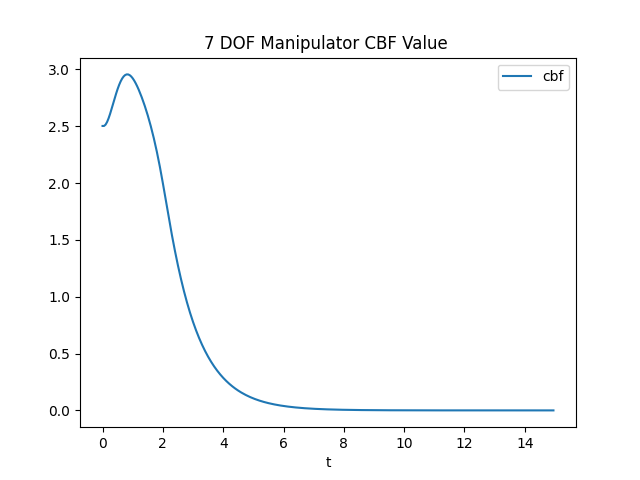
\includegraphics[width=0.45\textwidth]{Figures/Examples/7DOF/7DOFCBFValue.png}
    \caption{7-DOF Manipulator Barrier value}
    \label{fig:7dofbarriervalue2}
\end{figure}

\noindent Not only does the best effort controller breach the safety set, but it is unable to recover once it does. The CBF controller on the other hand maintains a safe configuration throughout. Figures \ref{fig:7dofnocbf2} and \ref{fig:7dofcbf2} show a model of this simulation both with and without CBF enforcement. The circle marks the 0.5m safety margin about the end effector desired by our barrier.

\begin{figure}[H]
    \centering
    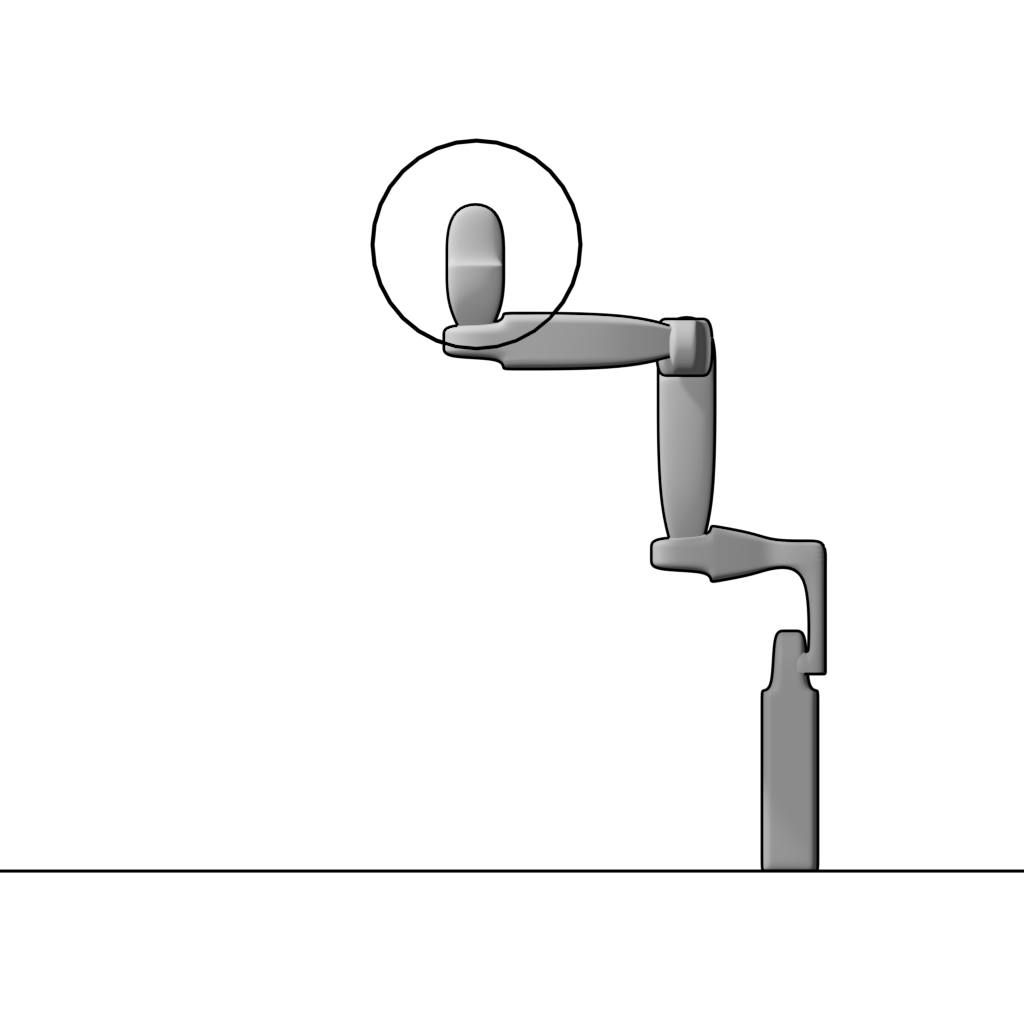
\includegraphics[width=0.3\textwidth]{Figures/Examples/7DOF/Frame0.png}
    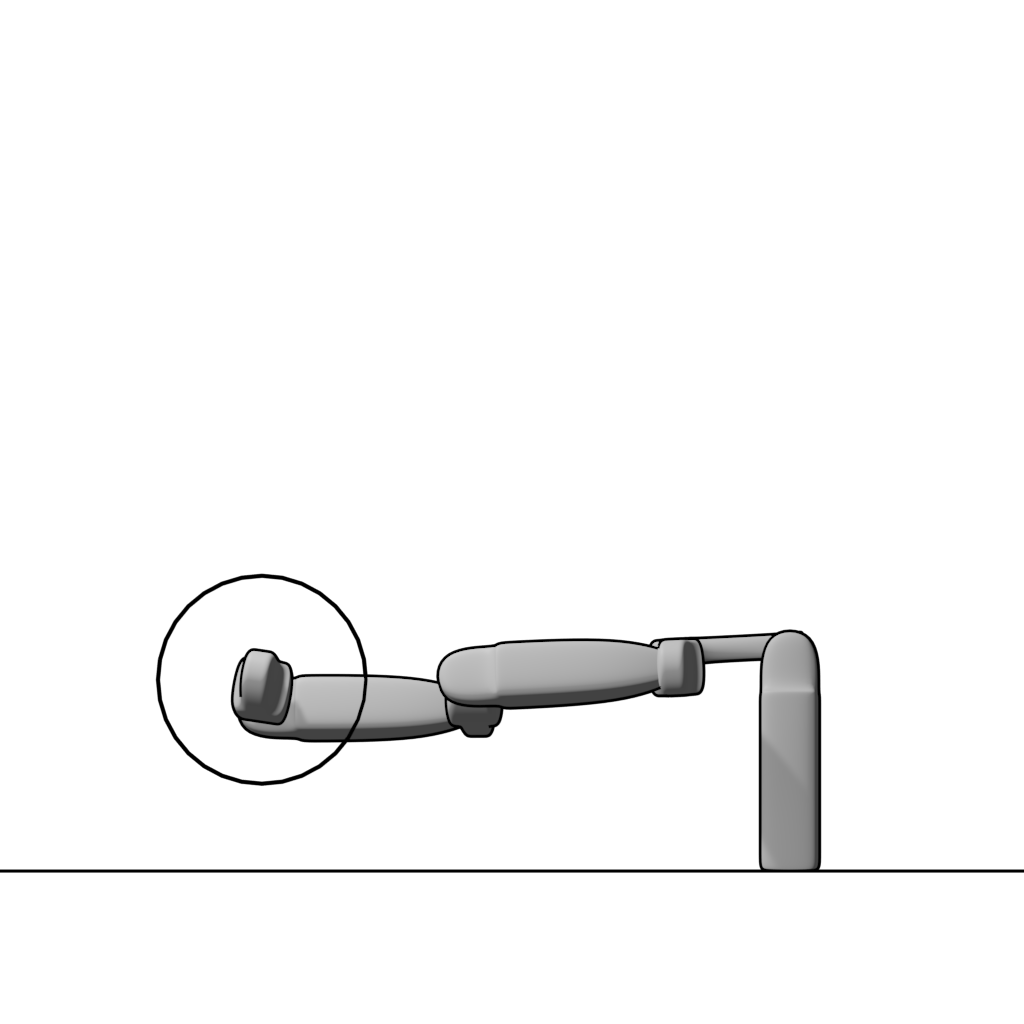
\includegraphics[width=0.3\textwidth]{Figures/Examples/7DOF/Frame56NOCBF.png}
    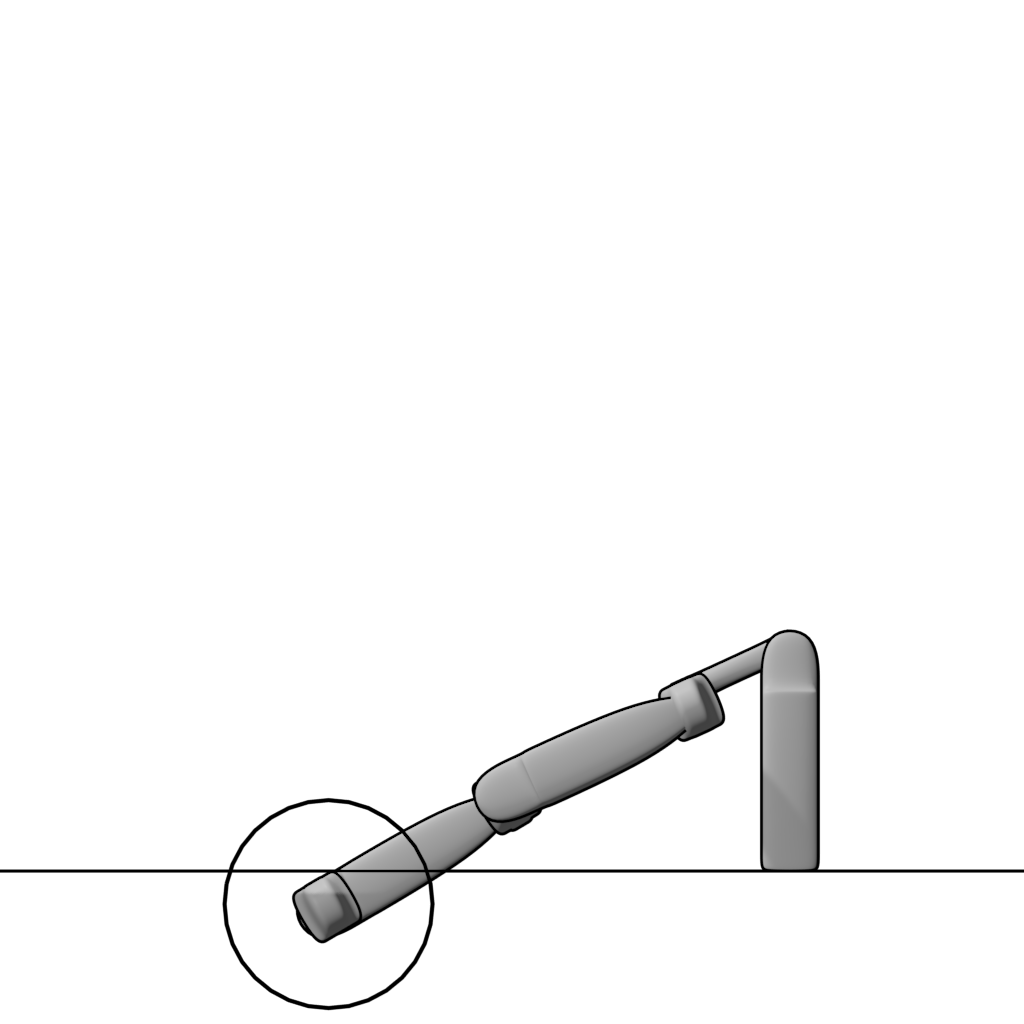
\includegraphics[width=0.3\textwidth]{Figures/Examples/7DOF/Frame300NOCBF.png}
    \caption{7-DOF Manipulator without CBF}
    \label{fig:7dofnocbf2}
\end{figure}

\begin{figure}[H]
    \centering
    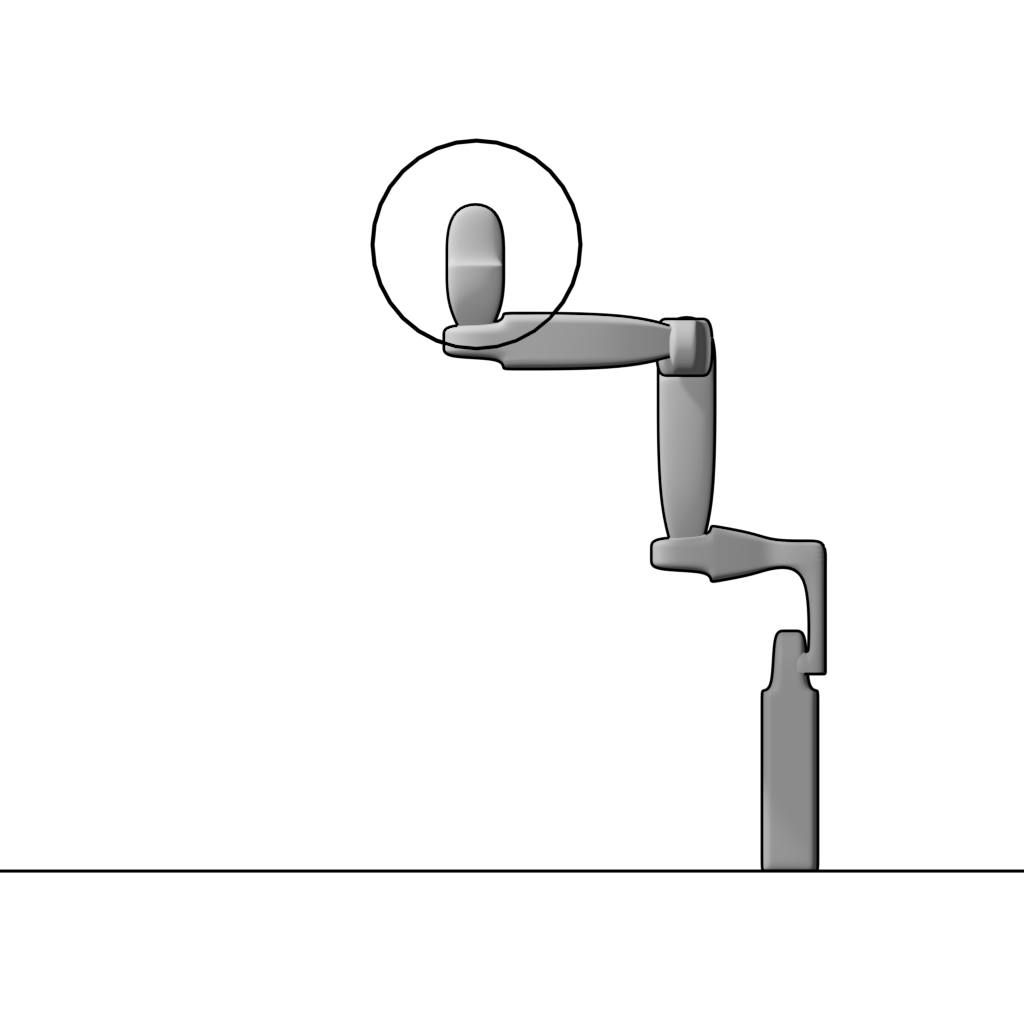
\includegraphics[width=0.3\textwidth]{Figures/Examples/7DOF/Frame0.png}
    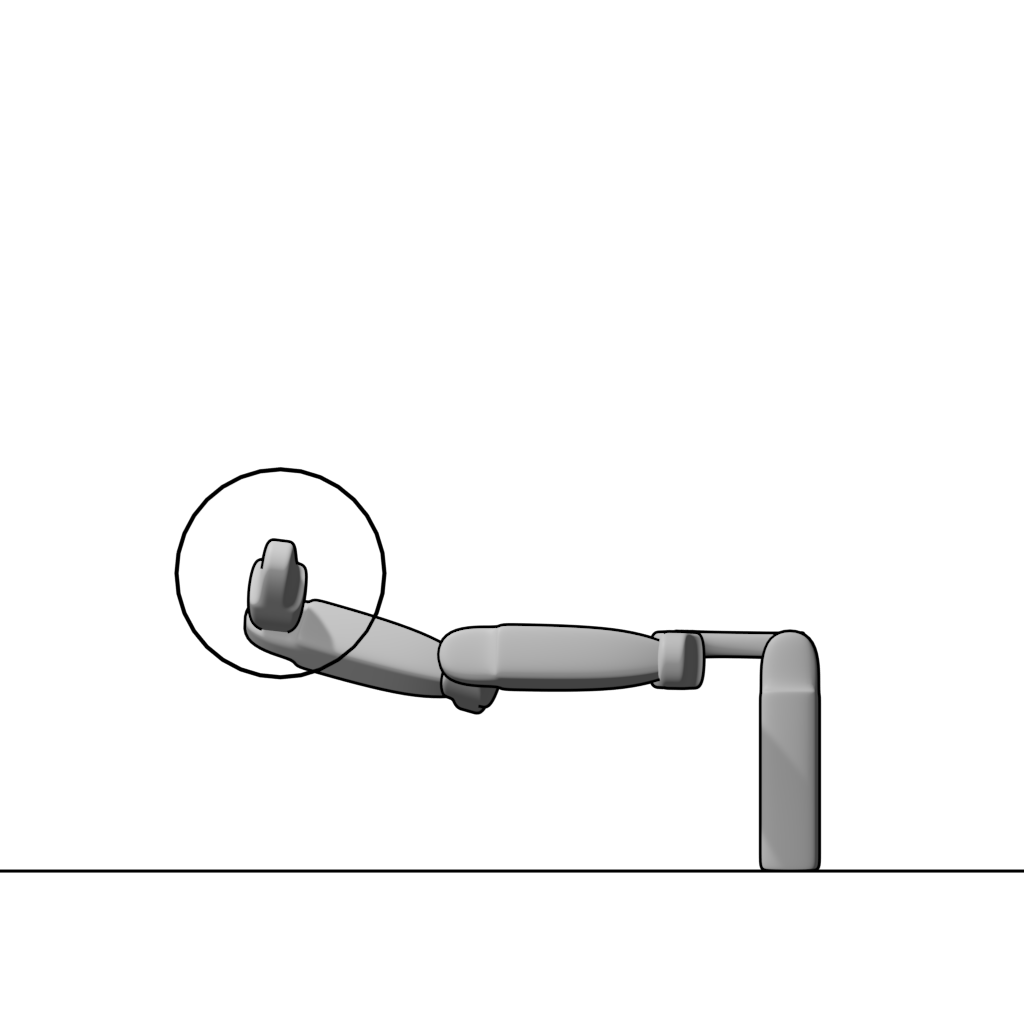
\includegraphics[width=0.3\textwidth]{Figures/Examples/7DOF/Frame56CBF.png}
    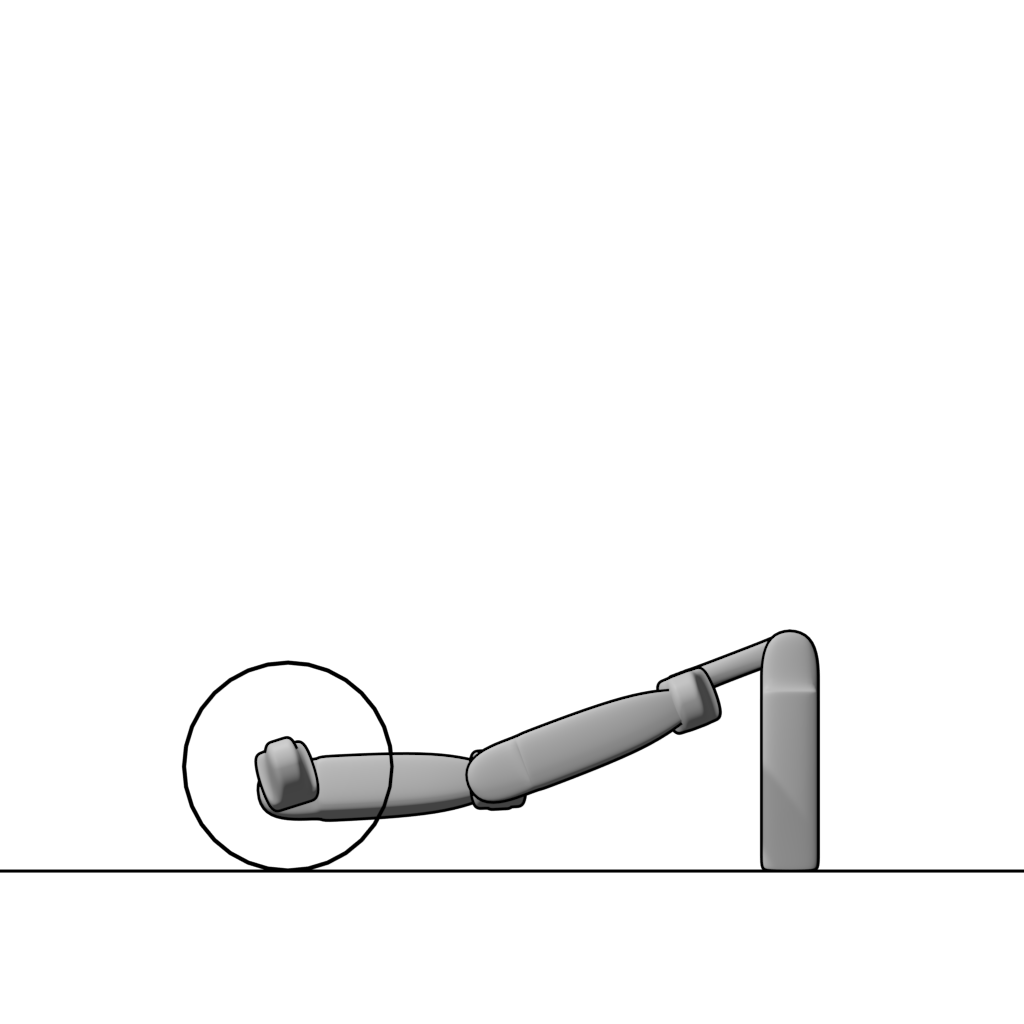
\includegraphics[width=0.3\textwidth]{Figures/Examples/7DOF/Frame300CBF.png}
    \caption{7-DOF Manipulator with CBF}
    \label{fig:7dofcbf2}
\section{Results}
\end{figure}